\subsection{Larger candidate sets improve gradient approximation}
\label{sec:coverage_gradient}

Truncating vocabulary support omits probability mass and changes token weights \citep{anshumann2025sparse,huang2026tailaware}. We measure coverage as the student probability retained by the student--teacher candidate intersection, $c_k(h)=\sum_{v\in S\cap T}p_\theta(v\mid h)$, and compare gradients.

\paragraph{Top-64 closely matches the full-vocabulary direction in Qwen.}
The intersection retains over 99.9\% of student probability on average, and its gradient direction is close to that of full-vocabulary supervision (Figure~\ref{fig:supervision_overview}b). Averaging 1, 16, and 64 token samples raises the mean gradient cosine from 0.54 to 0.87 to 0.97; top-64 exceeds 0.999 (Figure~\ref{fig:sampling_history_controls}a). This sampling control identifies finite-sample variation as one source of the directional difference.

\paragraph{Lower-coverage inputs retain appreciable gradient error in SmolLM.}
SmolLM3-3B measurements use the MixSFT initialization and its student after 500 updates of top-64 training with response averaging and three teachers for mathematics, code, and instruction following \citep{gao2026openmopddiagnosingfixingcapability}. Mean top-64 coverage is 97.42\% initially and 98.56\% after training; 8.42\% and 3.65\% of weighted prefixes retain less than 90\% mass (Figure~\ref{fig:smollm_supervision}a,b). Larger candidate sets reduce this low-coverage tail.

We compare gradients on typical prefixes, high-entropy prefixes, and prefixes with top-64 coverage below 99\%. Top-64 has 2.16--24.54\% relative gradient error against full-vocabulary supervision. Top-4 and top-8 produce larger errors in the evaluated batches (Figure~\ref{fig:smollm_supervision}d). Here relative error is the norm of the gradient difference divided by the full-vocabulary gradient norm, capturing both direction and magnitude. Larger candidate sets improve the approximation, with residual error at top-64.

\begin{figure}[t]
\centering
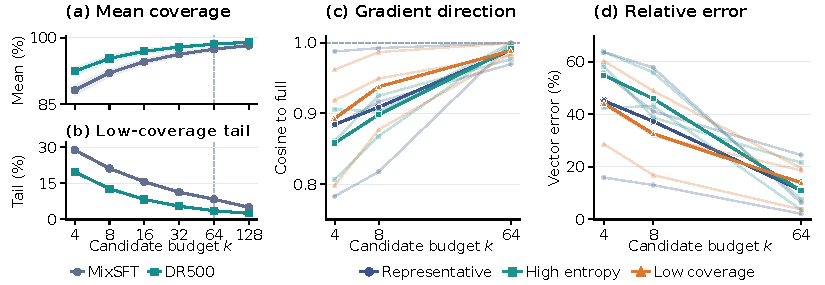
\includegraphics[width=\linewidth]{figures/layout_followup_20260918/smollm_supervision.pdf}
\caption{\textbf{Larger candidate sets improve coverage and gradient approximation in SmolLM.}
(a,b) Mean retained student probability and fraction of inputs below 90\% coverage; bands show response-cluster 95\% intervals. Dashed lines mark top-64.
(c,d) Gradient cosine and relative error against full-vocabulary supervision at the trained student. Groups comprise typical inputs, uncertain next-token predictions, and inputs with lower top-64 coverage; thin lines show batches and bold lines their means. MixSFT/DR500 denote the initialization/trained student.}
\label{fig:smollm_supervision}
\end{figure}

\paragraph{SmolLM capability scores also reveal changes below the aggregate.}
Sampled-token training with SGD raises MATH-500 accuracy from 50.60\% to 53.80\%. On AIME 2025, the initialization, the top-64/domain-token Adam student, and the sampled-token/response-averaged SGD student each solve four of 30 questions with eight samples per question; only one solved question is common to all three.
